\section{Team Coordination Algorithm}\label{sec:algo}
\noindent Our  MMDP model results in a very large search space,
even for small-sized problems. For example, with 8 responders and
17 tasks in a 50$\times$55 grid, the number of possible states is
more than $2\times 10^{400}$. Therefore, it is practically
impossible to compute the optimal solution. In such cases, we need
to consider approximate solutions that result in high quality
allocations.  To this end, we develop an
approximate solution using  the observation that responders first need to {\em cooperatively} select a
task to form a team with others (i.e., agree on who will do what),
and  that they can {\em independently} compute the best path to the task.
In our planning algorithm, we use this observation to decompose the
decision-making process into a hierarchical structure with two
levels: at the top level, a task planning algorithm is run for the
whole team to assign the best task to each responder given the
current state of the world; at the lower level, given a task, a
path planning algorithm is run by each responder to find the best
path to the task from his or her current location.

Furthermore, not all states of MMDPs are relevant to the problem
(e.g., if a responder gets injured, she is incapable of doing any
task in the future and therefore her state is irrelevant
to other responders) and we only need to consider the reachable
states given the current global state $S$ of the problem. Hence,
given the current state, we compute the policy online only for
reachable states. This saves a considerable amount of computation
because the size of the reachable states is usually much smaller
than the overall state space. For example, given the current
location of a responder, the one-step reachable locations are the 8
neighbouring locations plus the current locations, which are 9
locations out of the 50$\times$55 grid. Jointly, the reduction is
huge, from $(50\times 55)^8$ to $9^8$ for 8 responders. Another
advantage of online planning is that it allows us to refine the
model as more information is obtained or unexpected events happen.
For example, if the wind speed increases or the direction of wind
changes, the uncertainty about the radioactive cloud may increase.
If a responder becomes tired, the outcome of his or her actions may
be liable to greater uncertainty.

The main process of our online hierarchical planning algorithm is
outlined in Algorithm~\ref{alg:coordination}. The following
sections describe the procedures of each level in more detail.

\begin{algorithm}[t]
  \caption{Team Coordination}\small
  \label{alg:coordination}
  \Indm
  \KwIn{the MMDP model and the current state $s$.}
  \KwOut{the best joint action $\vec{a}$.}
  \Indp\BlankLine
  \tcp{The task planning}
  $\{ t_i \} \gets$ compute the best task for each responder $i\in I$ \;
  \ForEach{$i\in I$} {
    \tcp{The path planning}
    $a_i \gets$ compute the best path to task $t_i$ \;
  }
  \Return{$\vec{a}$}\vspace{-1mm}
\end{algorithm}


\subsection{Task Planning}
\label{sec:taskplanning}
\noindent As described in Section \ref{sec:model}, each responder
$p_i$ is of a specific type $\theta_i \in \Theta$ that determines which task
she can perform and  a task $t$ can only be completed by a team of
responders with the required types $\Theta_t$. If, at some point in
the execution of a plan, a responder $p_i$ is incapable of
performing a task (e.g., because she is tired or suffered a high
radiation dose), she will be removed from the set of responders
under consideration that is $I = I \setminus p_i$. This
information can be obtained from the state $s \in S$. When a task
is completed by a chosen team, the task is simply removed from the
set, that is $T = T\setminus t_k$ if $t_k$ has been completed.

Now, to capture the efficiency of groupings of responders at
performing tasks, we define  $C$ as a subset (or sub-team) of
responders, that is, $C \subseteq I$. Thus, we can identify all
possible teams $\{ C_{jk} \}$ for each task $t_j$ where $\{r_i
| p_i \in C_{jk}\} = \Theta_{t_j}$. Crucially, we define the value of
a team $v(C_{jk})$ that reflects the level of performance of a team
$C_k$ in performing task $t_k$.  Then, the goal of the task
planning algorithm is to assign a task to each team that maximises
the overall team performance given the current state $s$, i.e.,
$\sum_{j=1}^m v(C_j)$ where $C_j$ is a team for task $t_j$ and $\{
C_1, \cdots, C_m \}$ is a {\em partition} of $I$ ($\forall j\neq
j', C_j \bigcap C_{j'} = \emptyset$ and $\bigcup_{j=1}^m C_j=I$).
In what follows, we first detail the procedure to compute the value
of all teams that are valid in a given state and then proceed
to detail the main algorithm to allocate tasks. Note that these
algorithms take into account the uncertainties captured by the
transition function of the MMDP.


\subsubsection{Team Value Calculation}
\noindent The computation of values  $v(C_{jk})$ for each team
$C_{jk}$ is challenging because not all tasks can be completed by
one allocation (there are usually more tasks than responders) and
the policy after completing task $t_j$ must also be computed by the
agent, which is time-consuming given the number of states and joint
actions. Given this, we propose to estimate the value through
several simulations. This is much cheaper computationally because
we do not need to compute the complete policy in order to come up
with a good estimate of the team value though we may not be able to
evaluate all possible future outcomes. According to the central
limit theorem, as long as the number of simulations is sufficient
large, the estimated value will converge to the true team value.
The main process is outlined in Algorithm~\ref{alg:taskplanning}.
\begin{algorithm}[htbp]\small
  \caption{Team Value Calculation}
  \label{alg:taskplanning}
  \Indm
  \KwIn{the current state $s$,
  a set of unfinished tasks $T$,
  and a set of free responders $I$.}
  \KwOut{a task assignment for all responders.}
  \Indp\BlankLine
  $\{ C_{jk} \} \gets$ compute all possible teams of $I$ for
  $T$ \;
  \ForEach{$C_{jk} \in \{C_{jk}\}$}{
    \tcp{The $N$ trial simulations}
    \For{$i=1$ \KwTo $N$}{
        $(r, s') \gets$ simulate the process with the starting state $s$
        until task $k$ is completed by the responders in $C_{jk}$ \;
        \If{$s'$ is a terminal state} {
            $v_i(C_{jk}) \gets r$ \;
        } \Else {
            $V(s') \gets$ estimate the value of $s'$ with MCTS \;
            $v_i(C_{jk}) \gets r + \gamma V(s')$ \;
        }
    }
    $v(C_{jk}) \gets \frac{1}{N} \sum_{i=1}^{N} v_i(C_{jk})$ \;
  }
  \Return the task assignment computed by Equation~\ref{eq:cf}
\end{algorithm}

In each simulation of Algorithm~\ref{alg:taskplanning}, we first
assign the responders in $C_{jk}$ to task $t_j$ and run the
simulator starting from the current state $s$ (Line 4). After task
$t_j$ is completed, the simulator returns the sum of the rewards
$r$ and the new state $s'$ (Line 4). If all the responders in
$C_{jk}$ are incapable of doing other tasks (e.g., having received
too high a radioactive dose), the simulation is terminated (Line
5). Otherwise, we estimate the expected value of $s'$ using
Monte-Carlo Tree Search (MCTS)~\footnote{We could also use
multi-agent Q-learning as discussed in~\cite{proper2009solving}.}
(Line 8), which provides a good tradeoff between exploitation and
exploration of the policy space and has been shown to be efficient
for large MDPs~\cite{kocsis2006bandit}. After $N$ simulations, the
averaged value is returned as an approximation of the team value
(Line 10).

The basic idea of MCTS is to maintain a search tree where each node
is associated with a state $s$ and each branch is a task assignment
for all responders. To implement MCTS, the main step is to compute
an assignment for the free responders (a responder is free when she
is capable of doing tasks but not assigned to any task) at each
node of the search tree. This can be computed by
Equation~\ref{eq:cf} using the team values estimated by the UCB1
heuristic~\cite{auer2002finite} to balance exploitation and
exploration:
\begin{equation}\small
  v(C_{jk}) = \overline{v(C_{jk})} + c\sqrt{\frac{2N(s)}{N(s, C_{jk})}}
\end{equation}
where $\overline{v(C_{jk})}$ is the averaged value of team $C_{jk}$
at state $s$ so far, $c$ is a tradeoff constant, $N(s)$ is the
visiting frequency of state $s$, and $N(s, C_{jk})$ is the
frequency that team $C_{jk}$ has been selected at state $s$.
Intuitively, if a team $C_{jk}$ has higher averaged value of the
trials so far or is rarely selected in the previous visits, it has
higher chance to be selected in the next visit of the tree node.

As we assume that the role of a responder and the role requirements
of each task are static, we can compute all possible team values
offline. Therefore, in the online phase, we only need to filter out
the teams for completed tasks and those containing
incapacitated responders to compute the team set $\{ C_{jk} \}$.

\subsubsection{Coordinated Task Allocation}
\noindent Given the team values computed above, we then solve the
following optimisation problem to find the best solution:
\begin{equation}
  \begin{array}{lll}
    \max\limits_{x_{jk}} & \sum_{j, k} x_{jk} \cdot v(C_{jk}) & \\[2pt]
    \mbox{s.t.} & x_{jk} \in \{0, 1\} & \\[2pt]
    & \forall j, \sum_{k} x_{jk} \leq 1 & \mbox{(i)} \\[2pt]
    & \forall i, \sum_{j, k} \delta_i(C_{jk}) \leq 1 & \mbox{(ii)}
  \end{array}
  \label{eq:cf}
\end{equation}
where $x_{jk}$ is the boolean variable to indicate whether team
$C_{jk}$ is selected for task $t_j$ or not, $v(C_{jk})$ is the
characteristic function for team $C_{jk}$, and $\delta_i(C_{jk}) =
1$ if responder $p_i\in C_{jk}$ and 0 otherwise. In the
optimisation, constraint (i) ensures that a task $t_j$ is allocated
to at most one team (a task does not need more than one group of
responders) and constraint (ii) ensures that a responder $p_i$ is
assigned to only one task (a responder cannot do more than one task
at the same time). This is a standard Mixed Integer Linear Program
(MILP) that can be efficiently solved  using solvers such as IBM
ILOG's CPLEX or LPSOLVE.

\subsubsection{Adapting to Responder Requests}\label{sec:adaptive}
\noindent One important characteristic of our approach is that it can easily
incorporate the preferences of the responders. For example, if a
responder rejects a task allocated to it by the planning agent, we
simply filter out the teams for the task that contain this
responder. By so doing, the responder will not be assigned to the
task. Moreover, if a responder prefers to do the tasks with another
responder, we can increase the weights of the teams that
contain them in Equation~\ref{eq:cf} (by default, all teams
have identical weights of 1.0). Thus, our approach is adaptive to
 preferences of human responders.

\subsection{Path Planning}
\label{sec:pathplanning}

\noindent In the path planning phase, we compute the best path for
a responder to her assigned task. This phase is stochastic as there
are uncertainties in the radioactive cloud and the responders'
actions. We model this problem as a single-agent MDP that can be
defined as a tuple, $\mathcal{M}_i = \langle S_i, A_i, P_i, R_i
\rangle$, where: (1) $S_i = S_r \times S_{p_i}$ is the state space,
(2) $A_i$ is the set of $p_i$'s actions, (3) $P_i = P_r \times
P_{p_i}$ is the transition function, and (4) $R_i$ is the reward
function. In this level, responder $p_i$ only needs to consider the
states of the radioactive cloud $S_r$ and her own states $S_{p_i}$
and her moving actions. Similarly, the transition function only
needs to consider the spreading of the radioactive cloud $P_r$ and
the changes of her locations and health levels when moving in the
filed $P_{p_i}$, and the reward function only needs to consider the
cost of moving to a task and the penalty of receiving high
radiation doses. This is a typical MDP that can be solved by many
existing solvers (see the most recent
survey~\cite{kolobov2012planning}). We choose Real-Time Dynamic
Programming (RTDP)~\cite{barto1995learning} because it particularly
fits  our problem, that is, a goal-directed MDP with large number
of states. However, other approaches for Stochastic Shortest Path
MDPs could equally be used here.

There are several techniques we use to speed up the convergence of
RTDP. In our problem, the map is static. Thus, we can initialize
the value function $V(s)$ using the cost of the shortest path
between the current location to the task location on the map, which
can be computed offline without considering the radioactive cloud.
This helps RTDP quickly navigate among the obstacles (e.g.,
buildings, water pools, blocked roads) without getting trapped in
dead-ends during the search. Another speed up is also possible if,
when traversing the possible states, we only consider the
responder's current location and the neighbouring points. This will
further speed up the algorithm where the main bottleneck is the
huge state space.

\subsection{Simulation Results}

%\begin{figure}[htbp]
%  \centering
%  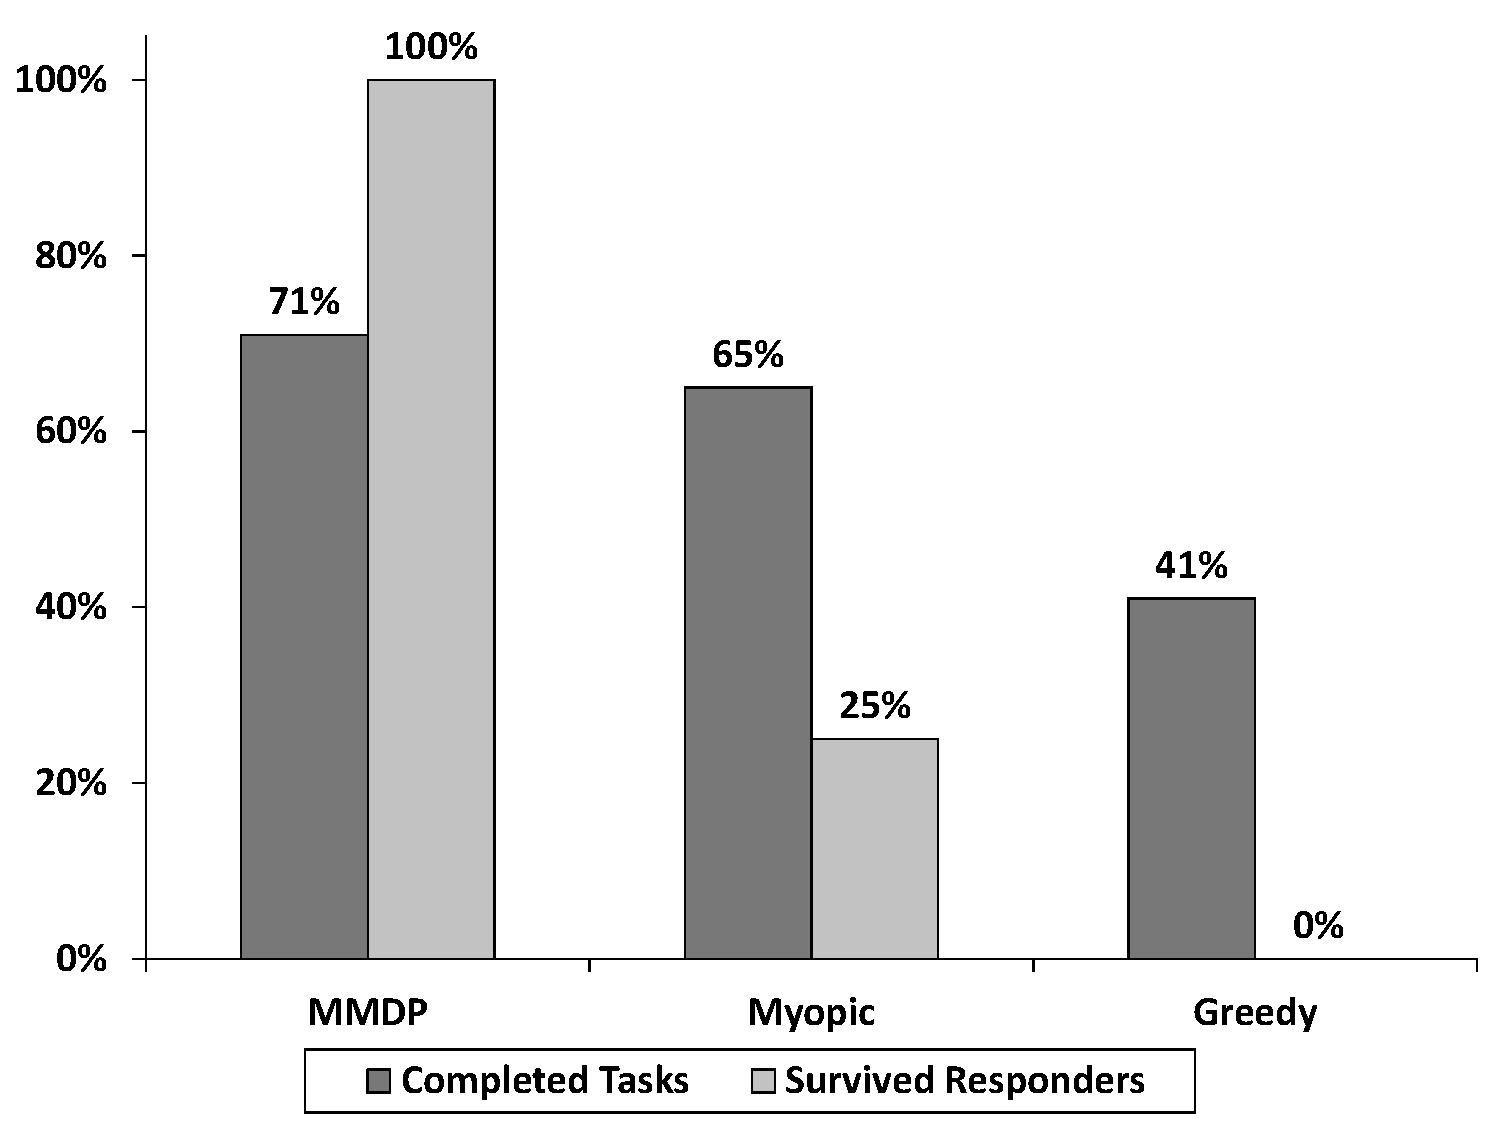
\includegraphics[width=0.8\linewidth]{simulation}
%  \caption{Experimental results for the MMDP, myopic, greedy
%  algorithms in simulation.}
%  \label{fig:simulation}
%\end{figure}


\noindent Before deploying our solution (as part of $PA$) to advise human responders, it is important to 
to test its performance to ensure it can return efficient solutions on simulations of the real-world problem. Given that there is no
comparable solution that takes into account uncertainty in team coordination for emergency response as we do,
we compare our algorithm with a greedy and a myopic method.
For each method, we use our path planning algorithm to compute the
path for each responder so that they can reach the task location as
fast as possible. In the greedy method, the responders are
uncoordinated and select the closest tasks that they can do. In the
myopic method, the responders are coordinated to select the tasks
but have no lookahead for the future tasks (Line 8 in
Algorithm~\ref{alg:taskplanning}). Table~\ref{tab:simulation} shows
the results for a problem with 17 tasks and 8 responders on a
50$\times$55 grid. Results show that our MMDP algorithm can complete
more tasks than the myopic and greedy methods (see Table \ref{tab:simulation}). More importantly,
our algorithm guarantees the safety of the responders, while in the
myopic method, only 25\% of the responders survive and in the
greedy method all responders are killed by the radioactive cloud.
More extensive evaluations are beyond the scope of this paper as
our focus here is on the use of the algorithm in a field deployment
to test how humans take up advice computed by the planning agent $PA$.
\begin{table}[htbp]
  \centering
  \caption{Experimental results for the MMDP, myopic, greedy
  algorithms in simulation.}
  \begin{tabular}{c|c|c|c}
   & MMDP & myopic & greedy \\
  \hline
  Completed Tasks & 71\% & 65\% & 41\% \\
  \hline
  Survived Responders & 100\% & 25\% & 0\% \\
  \end{tabular}
  \label{tab:simulation}\vspace{-3mm}
\end{table}
